\documentclass[11pt]{article}

\usepackage{graphicx, amsmath, amsfonts, amssymb, microtype, fullpage, url, algorithm, algorithmic, hyperref, longtable}
\newcommand{\argmax}{\operatornamewithlimits{argmax}}
\newcommand{\htmltag}{$\lt${htmltag}$\gt$}
\setlength{\parskip}{5pt}

\title{Project Report - Classification of Questions on Stackoverflow\\ Machine Learning, Fall 2012}
\author{Luke Vilnis, Annamalai Natarajan, Ariel Kobren}

\begin{document}
\sloppy

\maketitle

\section{Problem Statement}

``What is the best programming language?'' There are numerous answers
to this question but very little consensus among programmers as to the
correct one. While this question is interesting and can be fun to
discuss, it will only clutter a forum designed for objective questions.
In addition to opinion-based questions, other questions (e.g. off-topic questions unrelated to the
subject matter discussed on the forum) contribute noise to such forums. Automatically identifying these questions using machine learning is a difficult problem. We attempt to build a classifier and engineer features to separate inappropriate questions from the large number of valuable questions asked on one such website, StackOverflow.

 StackOverflow \cite{website:stackoverflow}, a web forum
for software and programming related questions,
has this exact problem. On StackOverflow, any user may ask any
question; those questions are subsequently answered by other users on
the website. StackOverflow has little infrastructure to restrict users
from posting irrelevant and/or subjective questions on the site. To
keep the forum clean and interesting, the website moderators (made up of employees and a
handful of influential users) have the ability to \emph{close} these
inappropriate questions. After a question is tagged as ``closed'', users cannot submit answers to it and it also is very unlikely to top any search results over questions. While the question
is still reachable, these measures effectively remove the question
from public discussion.

 Although StackOverflow has explicit policies regarding when
a question may be closed, these policies are largely
subjective. According to StackOverflow, a question may be closed if it
falls into one of these five categories:

\begin{itemize}
\item \textbf{Exact duplicate}: This category describes questions which may be reasonable and on-topic for StackOverflow, but have already appeared on the site.
\item \textbf{Off-topic}: Since StackOverflow is meant for software and programming related questions, questions that relate to domain-specific software packages or otherwise require the attention of specialists not likely to be found on StackOverflow are off-topic. An example of a question closed as off-topic is ``From the Brain imaging toolbox, AFNI, I see lots of activity in the Dorso Lateral pre-frontal cortex, does it mean that part of the brain is involved in activity A?''
\item \textbf{Not constructive}: Questions are closed as ``Not constructive'' when they solicit opinion, debate, arguments, polling, or extended discussion. Our opening question, ``What is the best programming language?'' is a common example.
\item \textbf{Not a real question}: When questions are ambiguous, vague, incomplete, overly broad or rhetorical. e.g. ``Sort HTML attributes with JavaScript'' - this user does not reveal the problem they encountered when attempting to perform this task.
\item \textbf{Too localized}: This comes up when the question pertains to a problem which occurs in very a specific setting and will not benefit future users of the forum. In general this is reserved for e.g. questions about very specific old versions of certain software and libraries.
\end{itemize}

\begin{figure}
\centering
\fbox{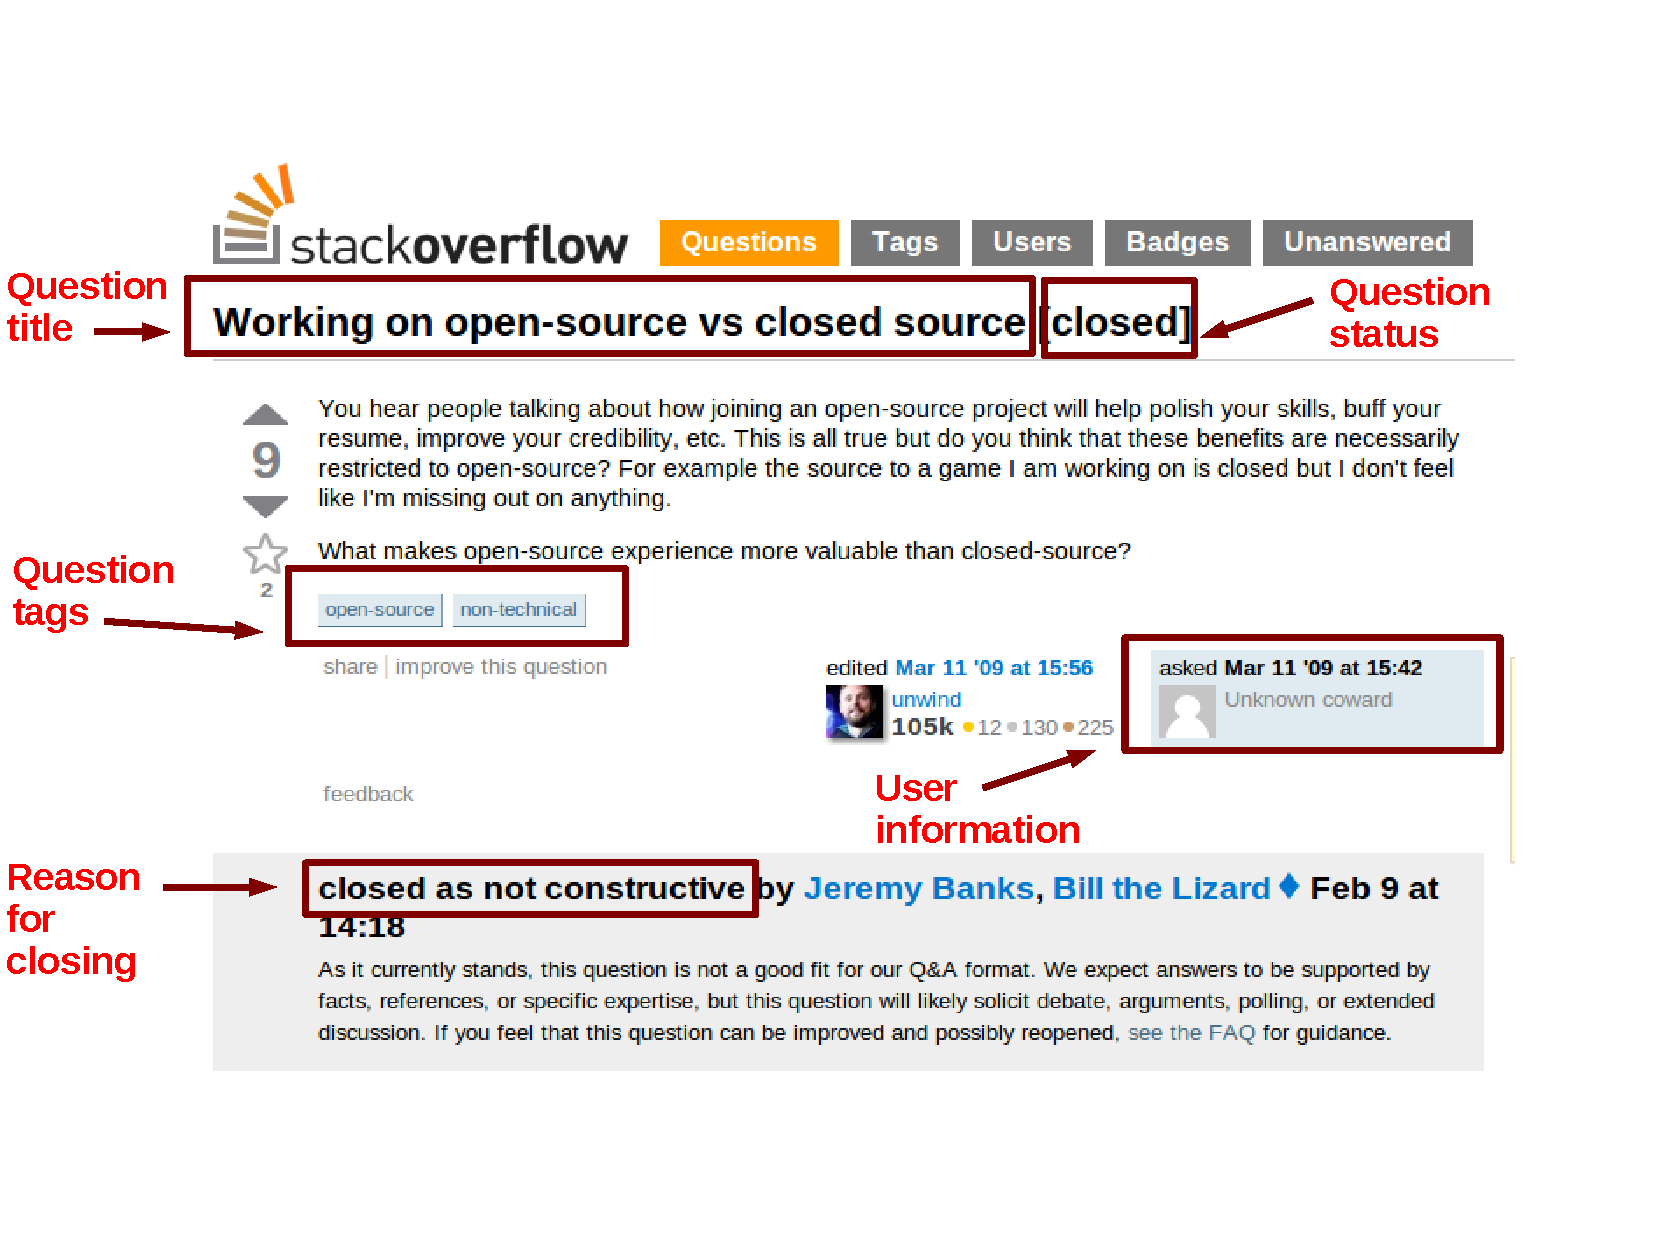
\includegraphics[width=4in,height=3.5in]{images/example_label.pdf}}
\caption{Sample closed question}
\label{fig:sample}
\end{figure}

 Figure \ref{fig:sample} shows a sample of closed question. An important consequence of this categorization of closed questions is that there is nothing essentially wrong with questions that are closed as ``Exact duplicate,'' aside from the fact that they were asked at the wrong point in time. Elimination of duplicate questions from the training data prevents us from confusing the classifier, which is attempting to identify structral commonalities between closed questions.

 Currently, closing questions is a manual process that
depends on the StackOverflow moderators paying close attention to every
question being asked. Closed questions also suffer from a class imbalance problem:
Stackoverflow estimates that only 6\% of its questions are closed each
year.

 In our project, we address the problem of detecting StackOverflow
questions that should be closed.  Using data gathered directly from
StackOverflow and various machine learning techniques, we train several classifiers to perform this detection automatically.

\section{Data set}
In our initial work, we use a data set collected using
Stackoverflow's \emph{StackExchange Data Explorer}
\cite{website:stackexchange}. This online tool
allows users to query raw data directly from
Stackoverflow. Specifically, we issued the following commands:

\begin{verbatim}
SELECT
  Posts.*,
  Users.Reputation
FROM Posts
  INNER JOIN Users ON Users.Id=Posts.OwnerUserId
WHERE
  Posts.PostTypeId=1 AND
  Posts.CreationDate > '20120801' AND
  Posts.ClosedDate IS NULL
ORDER BY
  Posts.CreationDate

SELECT
  Posts.*,
  Users.Reputation
FROM Posts
  INNER JOIN Users ON Users.Id=Posts.OwnerUserId
WHERE
  Posts.PostTypeId=1 AND
  Posts.CreationDate > '20120801' AND
  Posts.ClosedDate > '20100101'
ORDER BY
  Posts.CreationDate
\end{verbatim}

These two queries aim to retrieve all questions (PostTypeId=1 represents a question, as opposed to a comment or an answer) posted on StackOverflow on or after August 13$^{\textrm{th}}$, 2011 that: 1)
were closed on or after August 13$^{\textrm{th}}$ and 2) have not been
closed, respectively.  However, to prevent overloading the StackExchange servers, the Data
Explorer will not return more than 50,000 rows at a time.  Thus, after
issuing these two queries, we had collected a data set of 50,000
questions that had been closed (55MB) and 50,000 that were still open as of
query issue date (75MB).

The data was formatted as CSV files and contained the following
fields: \emph{Question Id}, \emph{PostTypeId},
\emph{AcceptedAnswerId}, \emph{ParentId}, \emph{CreationDate},
\emph{Score}, \emph{ViewCount}, \emph{Body}, \emph{OwnerUserId},
\emph{LastEditorUserId}, \emph{LastEditorDisplayName},
\emph{LastEditDate}, \emph{LastActivityData}, \emph{Title},
\emph{Tags}, \emph{AnswerCount}, \emph{CommentCount},
\emph{FavoriteCount}, \emph{ClosedDate}, \emph{CommunityOwnedDate} and
\emph{Reputation}. Of these fields, the fields that we worked
with were in our initial testing were:

\begin{enumerate}
  \item Body - the raw text of the question
  \item Tags - user provided question categories (e.g. Java,
    algorithms, etc.)
  \item ClosedDate - a non-null value here indicates that the post was
    closed.
    \item Reputation - the StackOverflow reputation of the user who
      asked the question
\end{enumerate}

\subsection{Pre-processing}
To get the data in workable form, a number of pre-processing steps
were required. First, the \emph{Body} field, which contained the text of
each question, was formatted as HTML and had to be
cleaned (i.e. HTML tags stripped). Additionally, images and code were
removed. Code presents several challenges: function and variable names are usually not meaningful, and the special symbols are hard to tokenize. The combination of these factors causes an explosion in the size of the vocabulary, as well as adding little more than noise to the data. However, the presence or absence of a given tag is usually an important feature (code examples or block quotations are an indication that the author put some time into the question). To capture this, we keep track of a list of tags found to use as features for our classifier.

An additional challenge that we faced was that the Data Explorer does
not give us access to the original text of a question, only the most
recent version, which includes moderator edits. This is obviously a
problem because moderator edits are highly correlated to ``Closed''
status, and using them as features would defeat the purpose of
building a classifier to automatically detect such questions. We used
several heuristics to detect such edits. Finally, any urls, which
often indicate a hyperlink to a similar question on Stackoverflow,
were removed.

Finally, we had to remove questions that were closed because they were
found to be duplicates of other questions on StackOverflow.  The
reason to do this is that questions being closed because they are
duplicates are generally \emph{good} questions that, in isolation, are
appropriate for StackOverflow. If we included these questions in the
data set, the classifier would get misinformation about what
constitutes a question deserving of being closed. In a real-world
system designed to automatically predict whether a question will be
closed, we suggest that first, the question be analyzed to determine
whether it is a duplicate and then, be analyzed by a system like ours.

Our complete list of preprocessing steps:

\begin{itemize}
\item Replace \{img\} tags with a the feature ``\#IMG\#''
\item Replace code with the tag ``\#CODE\#''
\item Replace URLs and add the feature ``\#URL\#''
\item Replace blockquotes and add the feature ``\#BLOCKQUOTE\#''
\item Remove indications of moderator comments
\item Remove duplicate questions
\end{itemize}

After being cleaned, the text of each question was tokenized using the Stanford NLP tokenizer.

\subsection{Features}

For each question, we extract two categories of features: one set of
features is extracted from the body of the question and the other from
the metadata. Metadata features are annotated with a specific tag
(e.g. ``\#TAG\#'') to prevent them from overlapping with vocabulary
words when added to the feature vector. The metadata features:

\begin{itemize}
  \item \textbf{Bucketed question length}: a collection of binary
    features taking the value $1$ if the number of characters in a
    question falls in a certain range.
  \item \textbf{Question tags}: we add each question tag (such as
    ``Java''), as well as conjunctions of tags and vocabulary words
    (these are useful to detect off-topic questions).
  \item \textbf{Title}: we add the unigrams contained in the question
    title to the respective feature vector.
  \item \textbf{Replacement Tags}: for each question, we strip out
    URLs, code, images and blockquotes and indicate their presence
    with a binary feature (e.g ``\#CODE\#'').
  \item \textbf{Reputation}: we bin the user reliability and add it as
    a feature.
\end{itemize}

Before extracting features from question bodies, first, each question
body was down-cased and tokenized. Then, we added the following
features:

\begin{itemize}
  \item \textbf{Unigrams}: we added a binary feature indicating the
    presence (or absence) of each unigram in our corpus.
  \item \textbf{Tag/Unigram Features}: we constructed the set of all
    tag-unigram conjuctions and added a binary feature for the
    presence of each.  This helps detect question that are off-topic.
  \item \textbf{Average TF-IDF}: we calculated the normalized TF-IDF
    \cite{wiki:tfidf} (term frequency inverse document frequency) of
    each word in each question. We averaged these scores over each
    question and added them as features. Normalized TF-IDF can be
    calculated as shown below:
    \begin{align*}
            tfidf(t,D) &= tf \cdot idf
    \end{align*}
    where:
    \begin{align*}
      tf(t,d) &= \frac{frequency(t,d)}{max\{frequency(w,d):w \in d\}}\\
      idf(t,D) &= \log\frac{|D|}{|\{d \in D : t \in d \}|}\\
    \end{align*}
\end{itemize}
Using all of the features described above, we constructed a set of
features with domain size of approximately 7.5 million.

\section{Software}

We made extensive use of third party software. In the pre-processing stage, we
used two different libraries.  First, to parse the CSV files
collected, we used a CSV parser called SuperCSV, written in Java
\cite{website:supercsv}. In addition, to tokenize the question bodies,
we made use of the Stanford NLP Library, also written in Java
\cite{stanfordnlp}.

To experiment with various classifiers, learning approaches, and
feature engineering, we used the FACTORIE library
\cite{mccallum09:factorie:}, written in Scala, that is developed at
UMass Amherst.  This library provides implementations of a variety of
textual pre-processing functions, classifiers, graphical models, and
learning algorithms. Additionally, two of the authors are committers
to this library, which made it easy to use, optimize, and fix bugs
found in the code. In fact, one of the authors was largely responsible
for the implementation of the classifiers and learning algorithms
(such as AdaGrad) that we used in this project.

In addition to third party software, we also wrote a large chunk of
the experiments ourselves.  The code that we wrote includes all of the
preprocessing, feature extraction and the code to run our experiments
with increasing dataset sizes.  All of this code is written in
Scala. In addition, we also wrote code in Matlab to generate our
plots.  All of this code is available on Github at:
https://github.com/lvilnis/StackExchange-Regression.

\section{Machine learning methods}
\subsection*{Classifiers}We tested 5 different classifiers on our data. Before we added more sophisticated features to our data, we found that Naive Bayes gave the best performance, but as we added features the log loss trained with the AdaGrad algorithm pulled ahead of the other strategies.
 \begin{itemize}
\item \textbf{Naive bayes}: The Naive Bayes classifier counts up occurences of features in each class, weighted by number of instances in the class. The weights learned represent basically the sum of all instances in the class, and new classifications are made by picking the class with the highest dot product. This extremely simple method gives a high-bias, low-variance classifier which can be effective for data sets where overfitting is a strong possibility, and as such worked surprisingly well on our data.
\item \textbf{L2-regularized Logistic regression}: We used FACTORIE's logistic regression implementation, which trains a log loss and l2-regularizer using LBFGS. Logistic regression attempts to learn a probabilistic classifier which makes the minimal amount of assumptions about the data. For example, there are no assumptions of independence between features.
\item \textbf{Liblinear SVM}: We used FACTORIE's implementation of Liblinear \cite{chang:08a}, a fast dual coordinate descent algorithm for learning SVM's with linear kernels. We used the L2 regularized, L1 loss version.
\item \textbf{AdaGrad with hinge loss and log loss}: We also tested two online algorithms against the other exact solvers, training hinge loss (SVM) and log loss (logistic regression) using the AdaGrad algoritm \cite{duchi:11a}. These loss functions were unregularized (did not include a penalty for the weights), but AdaGrad includes variable learning rates for each feature which has the effect of softly regularizing the weights. We found the online algorithms gave better performance over the exact solvers (the online strategy of regret minimization helps to prevent over-fitting), and made training times orders of magnitude faster.
\end{itemize}
\subsection*{Information gain.}We found \emph{information gain} \cite{wiki:infogain} to be a useful tool for cleaning the data of moderator edits and other features that proxy the ground truth. The information gain of a feature is a measure of the benefit of that feature for classification. We split the instances according to those possessing a feature and those lacking it, and measure the gain in entropy between the two resulting instance label distributions and the original distribution. If the two distributions are very dissimilar (i.e. lots of closed questions in one group, few in the other, compared to the original one), then that feature does a good job of distinguishing the two classes and has a high information gain. Features with extremely high information gain are probably too good to be true and the result of common patterns in moderator edits - we need to remove those features in our pre-processing. This is the formula for information gain:
\begin{equation*}
\begin{split}
InfoGain(f, P(x)) = H(P(x)) - \alpha*H(P(x|f=1)) - (1 - \alpha)*H(P(x|f=0))\\
\end{split}
\end{equation*}
Where $f$ is some binary feature, and $\alpha$ is the percentage of examples with the feature present.

\subsection*{AdaGrad}We used the AdaGrad \cite{duchi:11a} stochastic (sub)gradient descent algorithm to train our classifiers. AdaGrad (which we used with the Composite Mirror Descent update \cite{duchi:10a}) does proximal mirror descent with a squared Mahalanobis distance (under an adaptively estimated covariance matrix) as the proximal function. Keeping the covariance matrix diagonal for tractability, this is effectively a set of per-coordinate learning rates which are adjusted according to how much gradient AdaGrad has seen for a given feature. The form of AdaGrad which we used for this project has the following update equation:
\begin{equation*}
\begin{split}
G_i &\leftarrow G_i + \partial_i^2\\
w_i &\leftarrow w_i + \alpha \cdot \frac{1}{\rho + \sqrt{G_i}} \cdot \partial_i\\
\end{split}
\end{equation*}
Where $\textbf{G}$ is a vector of learning rates, $\textbf{w}$ is a vector of weights to be learned, $\alpha$ is the a learning rate, $\rho$ is a ridge for good conditioning, and $\partial$ is the (sub)gradient of the loss function.

\section{Results}
In our experiments, we aimed at measuring 2 quantities: 1) over test
set accuracy and 2) classifier accuracy as a function of the size of
the train set.  To do this, we split our data set randomly into 70\%
train and 30\% test.  We trained multiple classifiers on the training
data and measured their performance on predicting closed questions in
the test set.  We repeated this experiment 5 times, each time varying
the size of the overall data set used.  The sizes of our data sets
(measured in number of instances) were: 40,000, 80,000, 120,000,
160,000 and 200,000.

\begin{figure}
\centering
\fbox{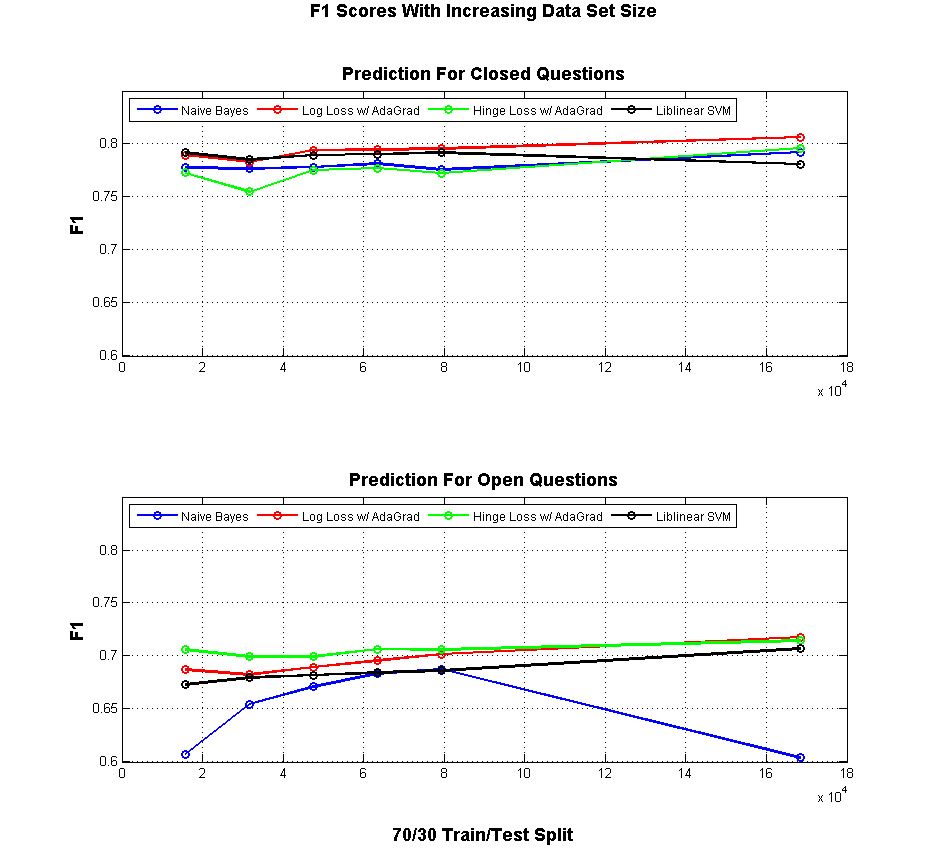
\includegraphics[width=6.5in,height=6in]{images/stackoverflow_results}}
\caption{Classifier accuracies in predicting closed questions}
\label{fig:results}
\end{figure}

As predicted, all of our classifiers improve as we increase the number
of the training instances. However, SVM did not perform as well as
expected.

\section{Discussion}

\subsection{Train Set Accuracy}
In almost all of our experiments, the accuracy achieved on the
training set was near 100\%.  Despite this, our results show our
accuracy on the held-out test set to be close to 75\%.  We believe
that the reason for this is that we didn't design features that
captured the essence of the problem we were trying to solve; that is,
our features didn't capture the entirety of what leads a question to
be ``closed.''

\subsection{Unhelpful Features}
In the process of refining our experiments, we tested the affect of a
few features that were not eventually included in training because
they did not improve overall accuracy on the test set. These features
include: bag of bigrams/trigrams and a bag of unigrams with their
TF-IDF scores.

\section{Future directions}
Though our project was largely successful, there are many
opportunities for extending the work.  As a first step, we're
interested repeating the same experiments with a much larger data
set. With more data, there is a chance that we will get better
classification performance. However, handling a larger data set poses
serious engineering problems.  The entire
StackOverflow data set contains 4.1 million questions - our experiments used only 100,000 (2.4\% of that).
Additional features could probably improve our performance even more.

We would also like to experiment with more question categories than just closed/open. For example, it would be a useful facility for users and moderators to be able to predict whether or not a certain question was likely to be answered. This could help users determine whether to add bounties to a question (which trade reputation from the asker to the answerer), or to move the question to some other, more domain-specific, StackExchange website. An extension to this would be to predict how long an asker could expect to wait before receiving an answer to their question.

We would also like to try some nonlinear classifiers, such as decision trees and random forests. We had trouble getting these to train in reasonable time on our data set, but this is probably more the fault of the inefficient implementation (written by one of the authors) than the algorithms themselves.

\section{Conclusion}
In this project, we attempted to train a classifier to predict whether
or not a given question would be closed on StackOverflow. Before
training, we needed to significantly pre-process the data. We
extracted multiple features from both the metadata and body of each
question and used them to train multiple classifiers for closed
question prediction. Among these trained classifiers, logistic
regression performed best with an overall accuracy of approximately
74\%. Moreover, we demonstrated that classifier performance
dramatically increases with the size of the training set.  While there
are many opportunities to extend this project, out project establishes
a foundation for ``appropriateness'' prediction of questions on online
forums.

\pagebreak
\bibliography{bib}{}
\bibliographystyle{plain}

\end{document}
